\section{Authentication System}
\label{prototype:AuthenticationSystem}
Following my research into authentication systems, I strived to implement the technical side of my learnings.

Much of the backend code is taken directly from the linked article as it should be - in the security industry using peer reviewed and certified code is crucial especially when, as a solo novice, developer this is one area where learning from mistakes isn't an acceptable outcome. 

After tweaking the code to work with my database system I quickly built an interface (made much easier by the frontend framework I had previously identified) which allowed me to test the system by logging in quickly and securely.

\begin{figure}[H]
    \centering
    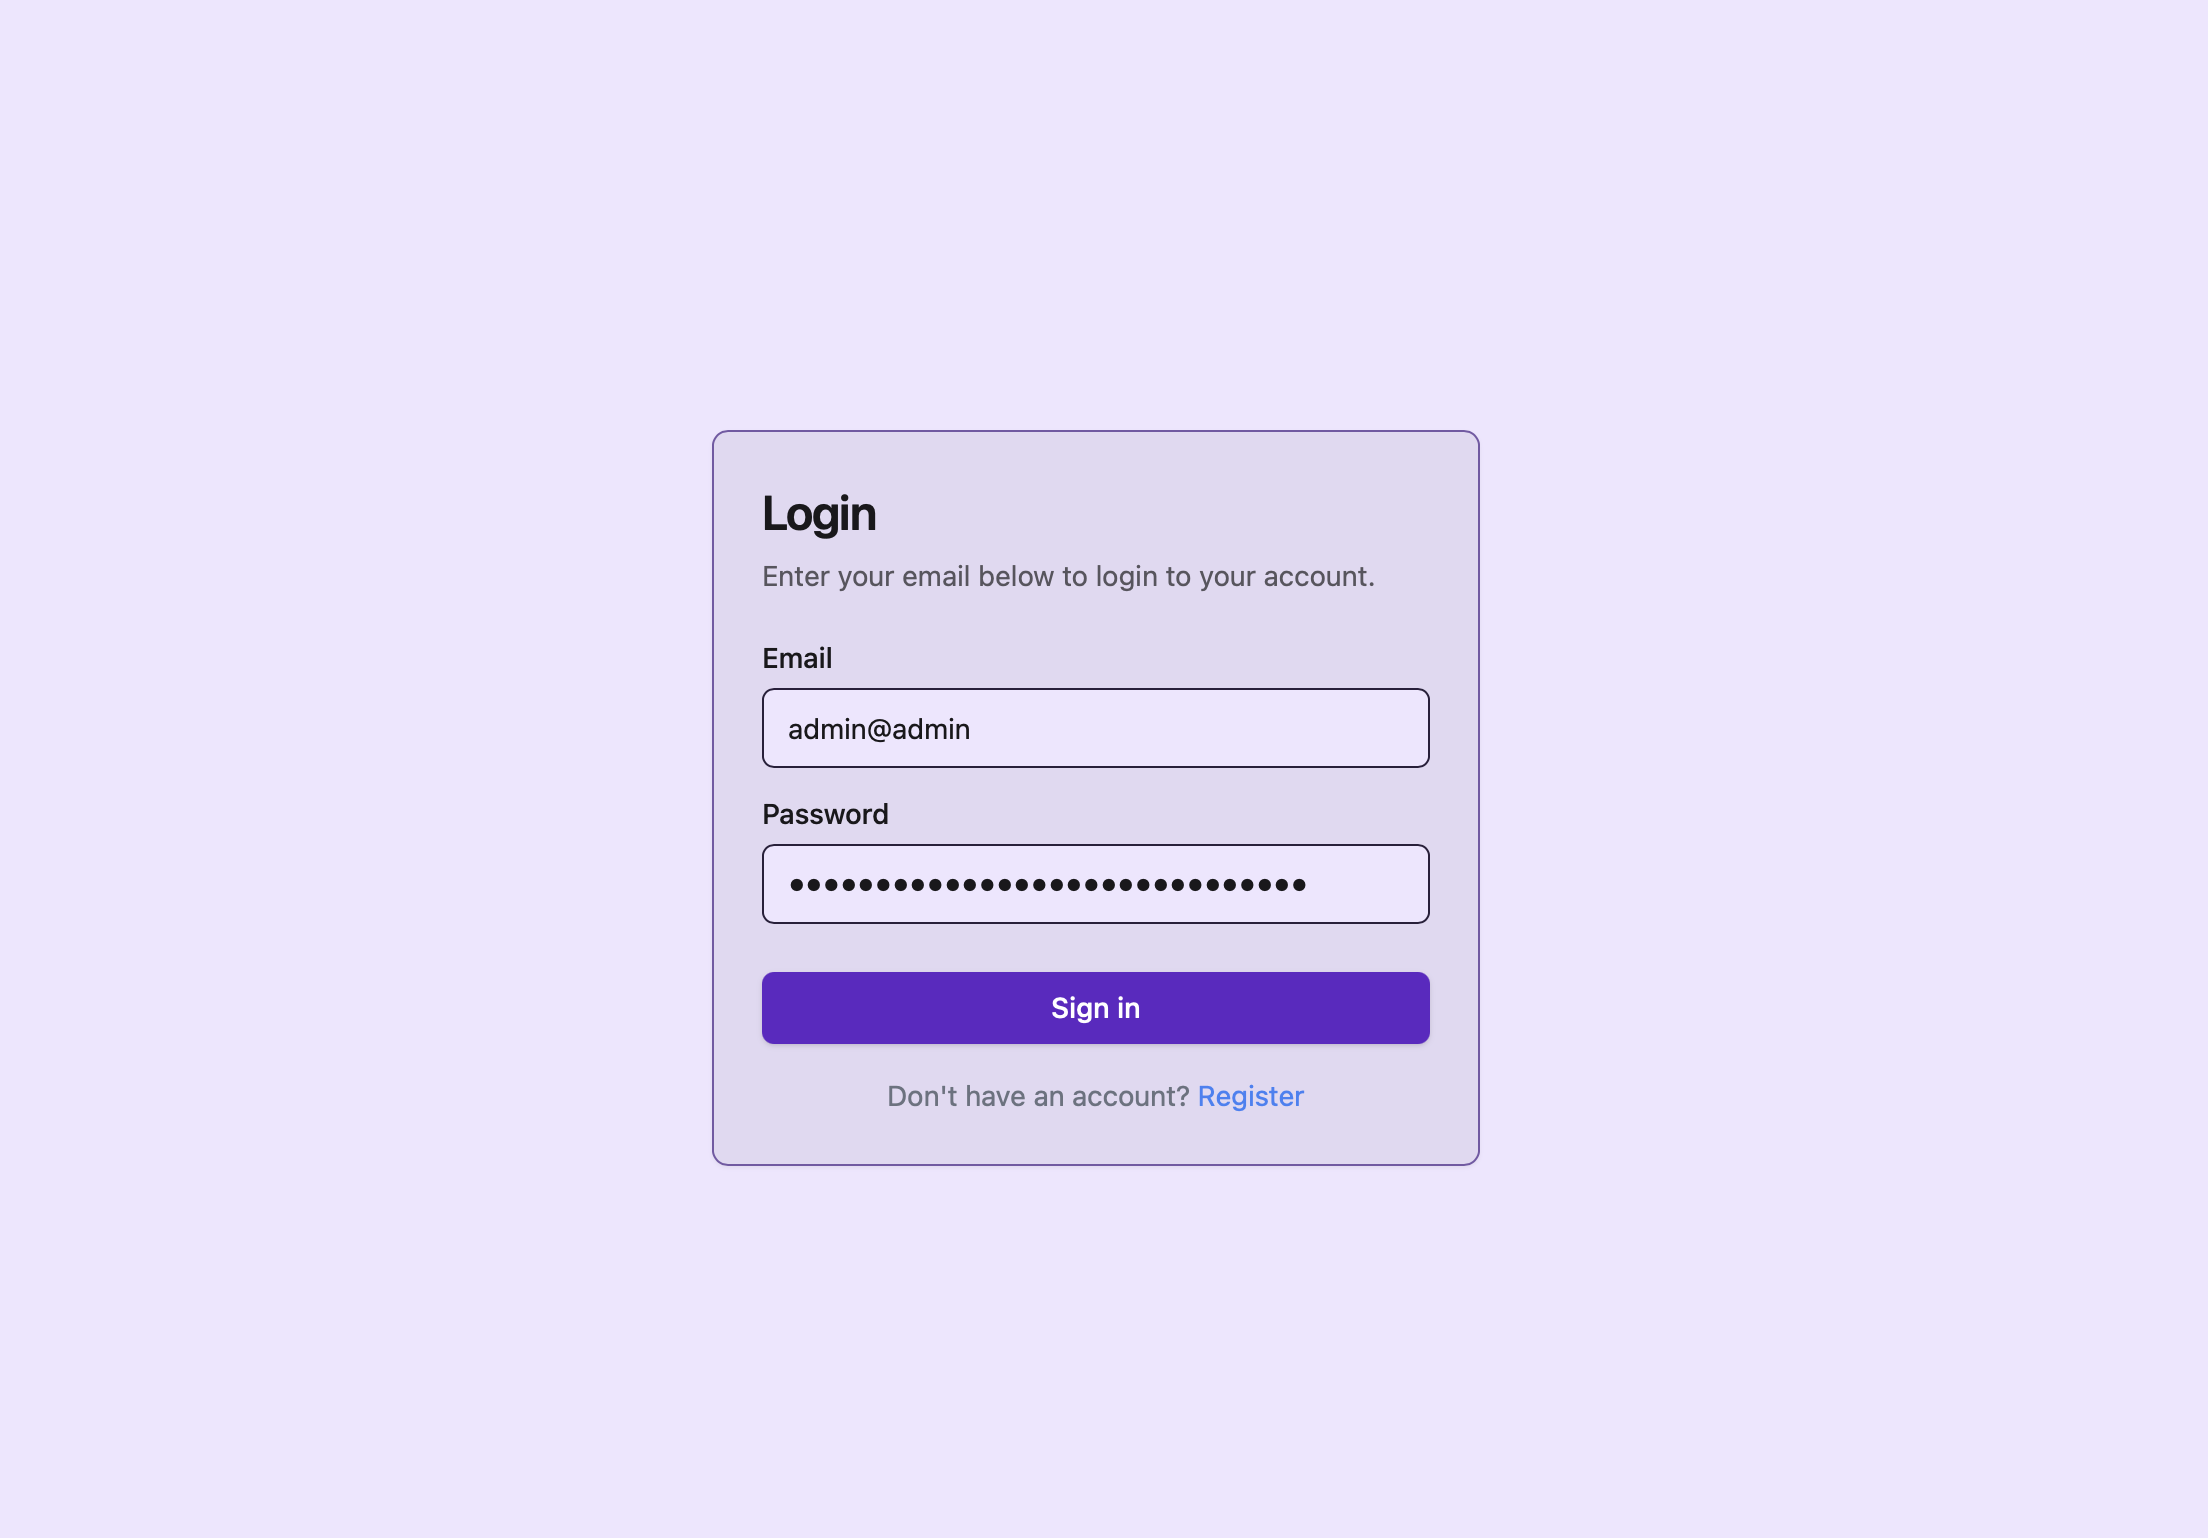
\includegraphics[width=0.8\textwidth]{Prototype/14_AuthenticationSystem/media/prototype.png}
    \caption{Prototype Login Interface}
\end{figure}


This Video clip demonstrates my login system working and taking me to the current dashboard once authenticated, you also see two password managers (Apple keychain \& Dashlane) recognise the requirements of the login page and offer to save details which makes the experience more seamless for the user - I did note however that whilst Dashlane picked up the website details, Apple keychain didn't and listed the platform as "(null)", I will research this further as this might effect a number of automated systems in the future.
